\chapter{Fuzzy Rough set based MCM}
Minimal Complexity Machine is a model which has advantages over SVM as described in Section \ref{mcmPaperReview}. In spite of the wide use of SVM it lacks in some area so as MCM. Hard margin SVMs deal with linearly separable data sets. However, if a high noise level causes a large overlap of the classes, then a separating hyperplane may not necessarily exist but noiseless data is not possible to get every time. To allow the possibility of violating constraints in the formulation of hard margin, slack variables were introduced and this version is known as soft margin SVMs. This relaxation can ensure that the soft margin SVMs will have a strong capacity to deal with noise. In many applications some input points may not necessarily be exactly assigned to either of the two classes. We know that SVM is sesnsitive to noise so it is possible that some data points corrupted by noises are less meaningful and it would be better if the machine should discard them. SVM lacks this kind
of capacity. The same issue comes with MCM. So Jaydeva \cite{FuzzyMCM} proposed an extension of MCM to fuzzy domain, in which a fuzzy membership  was assigned to every training sample. Outliers will be assigned small memberships so that they can contribute less to the final decision function. However, there is another interfering factor in the data set besides noise. Labeled training points consist of two parts : n-conditional features and the decision labels. The data is mostly collected by researchers. Owing to the limitation of human knowledge
and complexity of the objective world, it is possible that some conditional features may not necessarily have a close relationship with decision labels, and some key features related to decision labels might not be easily collected. This may lead to an inconsistency between the conditional features and decision labels, i.e., some samples have similar even same conditional feature values but different decision labels. For example, in earthquake prediction, with similarly observed conditional feature values, sometimes there is no earthquake, and sometimes an earthquake occurs. This statement implies that they may have superfluous conditional features but some key conditional features are likely to
be ignored in earthquake prediction. This kind of inconsistency can be observed in many practical conditions. Due to inconsistency, conditional features can only characterize the membership when a sample belongs to a certain decision class, and different samples may have different memberships. Fuzzy rough set based SVM \cite{frsvm} was introduced to address this problem.

In this section it is shown that how the MCM can be extended to fuzzy rough set theory, considering the fact that rough set considers the inconsistency of data. Preceding subsection explains the calculation of fuzzy rough set score , the formulation of FRMCM (Fuzzy Rough set based MCM) and the working of the model. The experimental results shown in the table \ref{fuzzymcmresult}.

\section{Fuzzy rough set score}
Kernel method is a way of introducing rough set into machine learning. A lower approximation operator in fuzzy transitive kernel based fuzzy rough sets can be used to compute membership for every training input. And then this membership can be used to reformulate hard margin minimal complexity machines into FRMCM. For calculating the score we have chosen Fuzzy rough set based Gaussian kernel, which is proved to fuzzy transitive kernel in \cite{FuzzyScore}.

The formulation of the score for each point x is shown in equation \ref{frScoreEqn} 
\begin{equation}\label{frScoreEqn}
s_x = min_{u \notin class(x)}\sqrt{1-(e^\frac{-||x-u||^2}{2\sigma^2})^2}
\end{equation}
where point u doesn't belong to class of x.


Fuzzy rough score of each training point is based on all the training point which belongs to the other class. This score shows how far away a point is from the other class i.e. those points which have high score are far distant from the nearest point of the other class. As shown in figure \ref{fig:frScore} the point encircled in red will have high score than the point encircled in green because of the distance from the nearest point of the other class. All scored are in between 0 and 1.

% You may add figures in the following manner.
\begin{figure}
\begin{center}	
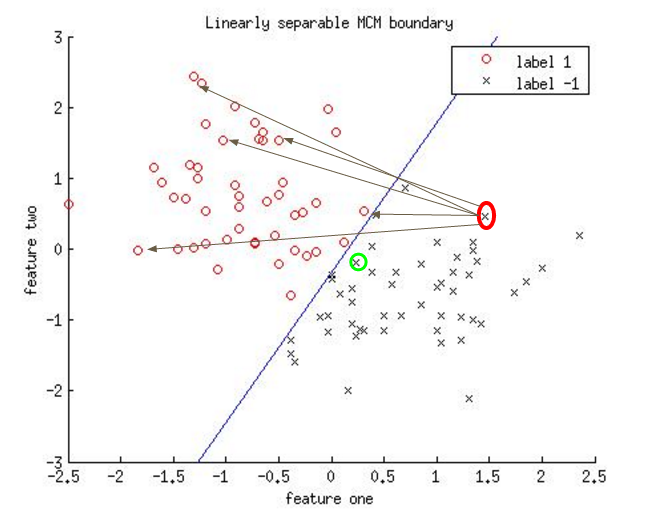
\includegraphics[scale=0.5]{scoreCalculation} 
\caption{Calculation Fuzzy Rough score}
\label{fig:frScore}
\end{center}
\end{figure}

\section{Fuzzy rough set based MCM}
Suppose $\{(x_1 , y_1 ),..., (x_M , y_M )\}$ is the training set and there are two classes A and B .We compute $s_i$ for all $x_i\epsilon A$ by equation \ref{frScoreEqn} where u are all those points who belong to class B. $s_i$ shows the degree of $x_i$ at which it belongs to A relative to the
conditional attributes. When we take $s_i$ into account for every $x_i$ , the optimal hyperplane problem is then reformulated as equation \ref{eqn:frmcm1}-\ref{eqn:frmcm4}

\begin{equation}\label{eqn:frmcm1}
min_{h,b,w,q}\:\: h + C\sum_i{s_i q_i}
\end{equation}
\begin{equation}\label{mceqn:frmcm2}
h \leq y_i(w^Tx_i+b)+ q_i \:\:\forall i={1, 2, .. M}
\end{equation}
\begin{equation}\label{eqn:frmcm3}
y_i(w^Tx_i +b) + q_i \geq s_i \:\:\forall i={1,2,.. M}
\end{equation}
\begin{equation}\label{eqn:frmcm4}
q_i \geq 0 \:\:\forall i={1, 2, ... M}
\end{equation}

continue from here.......
write about the prediction process and the working of FRMCM

\section{Where FRMCM outperforms other MCM}
TODO